\section*{15. Multivariate Models}\label{multivariate-models}
Review of notation from linear algebra:
\begin{itemize}[tightlist]
\item
  If \(x\) and \(y\) are vectors, then \(x^T y = \sum_{j} x_{j} y_{j}\).
\item
  If \(A\) is a matrix then \(\det(A)\) denotes the determinant of
  \(A\), \(A^T\) denotes the transpose of A, and \(A^{-1}\) denotes the
  inverse of \(A\) (if the inverse exists).
\item
  The trace of a square matrix \(A\), denoted by \(\text{tr}(A)\), is
  the sum of its diagonal elements.
\item
  The trace satisfies \(\text{tr}(AB) = \text{tr}(BA)\) and
  \(\text{tr}(A + B) = \text{tr}(A) + \text{tr}(B)\).
\item
  The trace satisfies \(\text{tr}(a) = a\) if \(a\) is a scalar.
\item
  A matrix \(\Sigma\) is positive definite if \(x^T \Sigma x > 0\) for
  all non-zero vectors \(x\).
\item
  If a matrix \(\Sigma\) is symmetric and positive definite, there
  exists a matrix \(\Sigma^{1/2}\), called the square root of
  \(\Sigma\), with the following properties:
  \begin{itemize}[tightlist]
  \item
\(\Sigma^{1/2}\) is symmetric
  \item
\(\Sigma = \Sigma^{1/2} \Sigma^{1/2}\)
  \item
\(\Sigma^{1/2} \Sigma^{-1/2} = \Sigma^{-1/2} \Sigma^{1/2} = I\)
    where \(\Sigma^{-1/2} = (\Sigma^{1/2})^{-1}\).
  \end{itemize}
\end{itemize}

\subsection*{15.1 Random Vectors}\label{random-vectors}
    Multivariate models involve a random vector \(X\) of the form
\[
X = \begin{pmatrix} X_{1} \\ \vdots \\ X_{k} \end{pmatrix}
\]
The mean of a random vector \(X\) is defined by
\[
\mu 
= \begin{pmatrix} \mu_{1} \\ \vdots \\ mu_{k} \end{pmatrix} 
= \begin{pmatrix} \EXP(X_{1}) \\ \vdots \\ \EXP(X_{k}) \end{pmatrix}
\]
The covariance matrix \(\Sigma\) is defined to be
\[
\Sigma = \VAR(X) = \begin{pmatrix}
\VAR(X_{1}) & \COV(X_{1}, X_{2}) & \cdots & \COV(X_{1}, X_{k}) \\
\COV(X_{2}, X_{1}) & \VAR(X_{2}) & \cdots & \COV(X_{2}, X_{k}) \\
\vdots & \vdots & \ddots & \vdots \\
\COV(X_{k}, X_{1}) & \COV(X_{k}, X_{2}) & \cdots & \VAR(X_{k})
\end{pmatrix}
\]
This is also called the variance matrix or the variance-covariance
matrix.

\textbf{Theorem 15.1}. Let \(a\) be a vector of length \(k\) and let
\(X\) be a random vector of the same length with mean \(\mu\) and
variance \(\Sigma\). Then \(\EXP(a^T X) = a^T\mu\) and
\(\VAR(a^T X) = a^T \Sigma a\). If \(A\) is a matrix with \(k\)
columns then \(\EXP(AX) = A\mu\) and
\(\VAR(AX) = A \Sigma A^T\).
Now suppose we have a random sample of \(n\) vectors:
\[
\begin{pmatrix}X_{11} \\ X_{21} \\ \vdots \\ X_{k1} \end{pmatrix}, \;
\begin{pmatrix}X_{21} \\ X_{22} \\ \vdots \\ X_{k2} \end{pmatrix}, \;
\cdots , \;
\begin{pmatrix}X_{1n} \\ X_{2n} \\ \vdots \\ X_{kn} \end{pmatrix}
\]
The sample mean \(\bar{X}\) is a vector defined by
\[
\bar{X} = \begin{pmatrix} \bar{X}_{1} \\ \vdots \\ \bar{X}_{k} \end{pmatrix}
\]
where \(\bar{X}_{i} = n^{-1} \sum_{j = 1}^{n} X_{ij}\). The sample
variance matrix is
\[
S = \begin{pmatrix} 
s_{11} & s_{12} & \cdots & s_{1k} \\
s_{12} & s_{22} & \cdots & s_{2k} \\
\vdots & \vdots & \ddots & \vdots \\
s_{1k} & s_{2k} & \cdots & s_{kk}
\end{pmatrix}
\]
where
\[
s_{ab} = \frac{1}{n - 1} \sum_{j = 1}^{n} (X_{aj} - \bar{X}_a) (X_{bj} - \bar{X}_b)
\]
It follows that \(\EXP(\bar{X}) = \mu\) and
\(\EXP(S) = \Sigma\).

\subsection*{15.2 Estimating the
Correlation}\label{estimating-the-correlation}
Consider \(n\) data points from a bivariate distribution
\[
\begin{pmatrix} X_{11} \\ X_{21}\end{pmatrix}, \;
\begin{pmatrix} X_{12} \\ X_{22}\end{pmatrix}, \;
\cdots \;
\begin{pmatrix} X_{1n} \\ X_{1n}\end{pmatrix}
\]
Recall that the correlation between \(X_{1}\) and \(X_{2}\) is
\[
\rho = \frac{\EXP((X_{1} - \mu) (X_{2} - \mu_{2}))}{\sigma_{1} \sigma_{2}}
\]
The sample correlation (the plug-in estimator) is
\[
\hat{\rho} = \frac{\sum_{i=1}^{n} (X_{1i} - \bar{X}_{1})(X_{2i} - \bar{X}_{2})}{s_{1} s_{2}}
\]
We can construct a confidence interval for \(\rho\) by applying the
delta method as usual. However, it turns out that we get a more accurate
confidence interval by first constructing a confidence interval for a
function \(\theta = f(\rho)\) and then applying the inverse function
\(f^{-1}\). The method, due to Fisher, is as follows. Define
\[
f(r) = \frac{1}{2} \left( \log(1 + r) - \log(1 - r)\right)
\]
and let \(\theta = f(\rho)\). The inverse of \(f\) is
\[
g(z) \equiv f^{-1}(z) = \frac{e^{2z} - 1}{e^{2z} + 1}
\]
Now follow the following steps:
\textbf{Approximate Confidence Interval for the Correlation}
\begin{enumerate}[tightlist,label={\arabic*.}]
\item
  Compute
\end{enumerate}
\[
\hat{\theta} = f(\hat{\rho}) = \frac{1}{2} \left( \log(1 + \hat{\rho}) - \log(1 - \hat{\rho})\right)
\]
\begin{enumerate}[tightlist,label={\arabic*.},resume]
\item
  Compute the approximate standard error of \(\hat{\theta}\) which can
  be shown to be
\end{enumerate}
\[
\widehat{\SE}(\hat{\theta}) = \frac{1}{\sqrt{n - 3}}
\]
\begin{enumerate}[tightlist,label={\arabic*.},resume]
\item
  An approximate \(1 - \alpha\) confidence interval for
  \(\theta = f(\rho)\) is
\end{enumerate}
\[
(a, b) \equiv \left(\hat{\theta} - \frac{z_{\alpha/2}}{\sqrt{n - 3}}, \; \hat{\theta} + \frac{z_{\alpha/2}}{\sqrt{n - 3}} \right)
\]
\begin{enumerate}[tightlist,label={\arabic*.},resume]
\item
  Apply the inverse transformation \(f^{-1}(z)\) to get a confidence
  interval for \(\rho\):
\end{enumerate}
\[
\left( \frac{e^{2a} - 1}{e^{2a} + 1}, \frac{e^{2b} - 1}{e^{2b} + 1} \right)
\]

\subsection*{15.3 Multinomial}\label{multinomial}
Review of Multinomial distribution: consider drawing a ball from an urn
that has \(n\) balls of \(k\) colors. Let \(p = (p_{1}, \dots, p_{k})\)
where \(p_{j} \geq 0\) are the probabilities of drawing (with replacement)
a ball of each color; \(\sum_{j} p_{j} = 1\). Draw \(n\) times and let
\(X = (X_{1}, \dots, X_{n})\) where \(X_{j}\) is the number of times that
color \(j\) appeared; so \(\sum_{k} X_{k} = n\). We say \(X\) has a
Multinomial(\(n\), \(p\)) distribution. The probability function is
\[
f(x; p) = \binom{n}{x_{1} \dots x_{k}} p_{1}^{x_{1}}\dots p_{k}^{x_{k}}
\]
where
\[
\binom{n}{x_{1} \dots x_{k}} = \frac{n!}{x_{1}! \dots x_{k}!}
\]

\textbf{Theorem 15.2}. Let \(X \sim \text{Multinomial}(n, p)\). Then the
marginal distribution of \(X_{j}\) is
\(X_{j} \sim \text{Binomial}(n, p_{j})\). The mean and variance of \(X\) are
\[
\EXP(X) = \begin{pmatrix} np_{1} \\ \vdots \\ np_{k} \end{pmatrix}
\]
and
\[
\VAR(X) = \begin{pmatrix}
np_{1}(1 - p_{1}) & -np_{1}p_{2} & \cdots & -np_{1}p_{k} \\
-np_{1}p_{2} & np_{2}(1 - p_{2}) & \cdots & -np_{2}p_{k} \\
\vdots & \vdots & \ddots & \vdots \\
-np_{1}p_{k} & -np_{2}p_{k} & \cdots & -np_{k}(1 - p_{k})
\end{pmatrix}
\]
\textbf{Proof}. That \(X_{j} \sim \text{Bimomial}(n, p_{j})\) follows
easily. Hence \(\EXP(X_{j}) = np_{j}\) and
\(\VAR(X_{j}) = np_{j}(1 - p_{j})\).
To compute \(\COV(X_{i}, X_{j})\), notice that
\(X_{i} + X_{j} \sim \text{Binomial}(n, p_{i} + p_{j})\), so
\(\VAR(X_{i} + X_{j}) = n (p_{i} + p_{j}) (1 - p_{i} - p_{j})\). On the other
hand, decomposing the sum of the random variables on the variance,
\begin{align*}
\VAR(X_{i} + X_{j}) &= \VAR(X_{i}) + \VAR(X_{j}) + 2 \COV(X_{i}, X_{j}) \\
&= np_{i}(1 - p_{i}) + np_{j}(1 - p_{j}) + 2 \COV(X_{i}, X_{j})
\end{align*}
Equating both expressions and isolating the covariance we get
\(\COV(X_{i}, X_{j}) = -np_{i}p_{j}\).

\textbf{Theorem 15.3}. The maximum likelihood estimator of \(p\) is
\[
\hat{p} 
= \begin{pmatrix} \hat{p}_{1} \\ \vdots \\ \hat{p}_{k} \end{pmatrix}
= \begin{pmatrix} \frac{X_{1}}{n} \\ \vdots \\ \frac{X_{k}}{n} \end{pmatrix}
= \frac{X}{n}
\]
\textbf{Proof}. The log-likelihood (ignoring a constant) is
\(\ell(p) = \sum_{j} X_{j} \log p_{j}\). When we maximize it we need to be
careful to enforce the constraint that \(\sum_{j} p_{j} = 1\). Using
Lagrange multipliers, instead we maximize
\[
A(p) = \sum_{j=1}^{k} X_{j} \log p_{j} + \lambda \left( \sum_{j=1}^{k} p_{j} - 1 \right)
\]
But
\[
\frac{\partial A(p)}{\partial p_{j}} = \frac{X_{j}}{p_{j}} + \lambda
\]
Setting it to zero we get \(\hat{p}_{j} = - X_{j} / \lambda\). Since
\(\sum_{j} \hat{p}_{j} = 1\) we get \(\lambda = -n\) and so
\(\hat{p}_{j} = X_{j} / n\), which is our result.
Next we want the variance of the MLE. The direct approach is to compute
the variance matrix of \(\hat{p}\) directly:
\(\VAR(\hat{p}) = \VAR(X / n) = n^{-2} \VAR(X)\), so
\[
\VAR(\hat{p}) = \frac{1}{n} \begin{pmatrix}
p_{1}(1 - p_{1}) & -p_{1}p_{2} & \cdots & -p_{1}p_{k} \\
-p_{1}p_{2} & p_{2}(1 - p_{2}) & \cdots & -p_{2}p_{k} \\
\vdots & \vdots & \ddots & \vdots \\
-p_{1}p_{k} & -p_{2}p_{k} & \cdots & p_{k}(1 - p_{k})
\end{pmatrix}
\]

\subsection*{15.4 Multivariate Normal}\label{multivariate:normal}
Recall the definition of the multivariate normal. Let
\[
Z = \begin{pmatrix} Z_{1} \\ \vdots \\ Z_{k} \end{pmatrix}
\]
where \(Z_{1}, \dots, Z_{k} \sim N(0, 1)\) are independent. The density of
\(Z\) is
\[
f(z) = \frac{1}{(2\pi)^{k / 2}} \exp \left\{ -\frac{1}{2} \sum_{j=1}^{k} z_{j}^{2} \right\} = \frac{1}{(2\pi)^{k / 2}} \exp \left\{ -\frac{1}{2} z^T z \right\}
\]
The variance matrix of \(Z\) is the identity matrix \(I\). We write
\(Z \sim N(0, I)\) where it is understood that \(0\) is a vector of
\(k\) zeroes. We say \(Z\) has a standard multivariate Normal
distribution.
More generally, a vector \(X\) has a multivariate Normal distribution,
denoted by \(X \sim N(\mu, \Sigma)\), if its density is
\[
f(x; \mu, \Sigma) = \frac{1}{(2 \pi)^{k / 2} \det(\Sigma)^{1/2}} \exp \left\{ -\frac{1}{2} (x - \mu)^T \Sigma^{-1} (x - \mu)\right\}
\]
where \(\mu\) is a vector of length \(k\) and \(\Sigma\) is a
\(k \times k\) symmetric, positive definite matrix. Then
\(\EXP(X) = \mu\) and \(\VAR(X) = \Sigma\). Setting
\(\mu = 0\) and \(\Sigma = I\) gives back the standard Normal.

\textbf{Theorem 15.4}. The following properties hold:
\begin{enumerate}[label={\arabic*.}]
\item
  If \(Z \sim N(0, 1)\) and \(X = \mu + \Sigma^{1/2} Z\) then
  \(X \sim N(\mu, \Sigma)\).
\item
  If \(X \sim N(\mu, \Sigma)\), then
  \(\Sigma^{-1/2}(X - \mu) \sim N(0, 1)\).
\item
  If \(X \sim N(\mu, \Sigma)\) and \(a\) is a vector with the same
  length as \(X\), then \(a^T X \sim N(a^T \mu, a^T \Sigma a)\).
\item
  Let \(V = (X - \mu)^T \Sigma^{-1} (X - \mu)\). Then
  \(V \sim \xi_{k}^{2}\).
\end{enumerate}
Suppose we partition a random Normal vector \(X\) into two parts
\(X = (X_a, X_b)\). We can similarly partition the mean
\(\mu = (\mu_a, \mu_b)\) and the variance
\[
\Sigma = \begin{pmatrix} 
\Sigma_{aa} & \Sigma_{ab} \\
\Sigma_{ba} & \Sigma_{bb}
\end{pmatrix}
\]

\textbf{Theorem 15.5}. Let \(X \sim N(\mu, \Sigma)\). Then:
\begin{enumerate}[tightlist,label={\arabic*.}]
\item
  The marginal distribution of \(X_a\) is
  \(X_a \sim N(\mu_a, \Sigma_{aa})\).
\item
  The conditional distribution of \(X_b\) given \(X_a = x_a\) is
\end{enumerate}
\[
X_b | X_a = x_a \sim N(\mu(x_a), \Sigma(x_a))
\]
where
\begin{align*}
\mu(x_a) &= \mu_b + \Sigma_{ba} \Sigma_{aa}^{-1} (x_a - \mu_a) \\
\Sigma(x_a) &= \Sigma_{bb} - \Sigma_{ba}\Sigma_{aa}^{-1}\Sigma_{ab}
\end{align*}

\textbf{Theorem 15.6}. Given a random sample of size \(n\) from a
\(N(\mu, \Sigma)\), the log-likelihood (up to a constant not depending
on \(\mu\) or \(\Sigma\)) is given by
\[
\ell(\mu, \Sigma) = -\frac{n}{2} (\bar{X} - \mu)^T \Sigma^{-1} (\bar{X} - \mu) - \frac{n}{2} \text{tr} \left( \Sigma^{-1}S \right) - \frac{n}{2} \log \det \left( \Sigma \right)
\]
The MLE is
\[
\hat{\mu} = \bar{X} 
\quad \text{and} \quad
\hat{\Sigma} = \left( \frac{n - 1}{n} \right) S
\]

\subsection*{15.5 Appendix}\label{appendix:multivariate}
\textbf{Proof of Theorem 15.6}. Let the \(i\)-th random vector be
\(X^{i}\). The log-likelihood is
\[
\ell(\mu, \Sigma) = \sum_{i = 1}^{k} f(X^{i}; \mu, \Sigma) 
= -\frac{kn}{2} \log ( 2\pi ) - \frac{n}{2} \log \det \left( \Sigma \right)
- \frac{1}{2} \sum_{i=1}^{k} (X^{i} - \mu)^T \Sigma^{-1} (X^{i} - \mu)
\]
Now,
\begin{align*}
\sum_{i=1}^{k} (X^{i} - \mu)^T \Sigma^{-1} (X^{i} - \mu) &=
\sum_{i=1}^{k} \left[ (X^{i} - \overline(X)) + (\bar{X} - \mu) \right]^T \Sigma^{-1} \left[(X^{i} - \bar{X}) + (\bar{X} - \mu) \right] \\
&= \sum_{i=1}^{k} [(X^{i} - \bar{X})^T\Sigma^{-1}(X^{i} - \bar{X})]
+ n (\bar{X} - \mu)^T \Sigma^{-1} (\bar{X} - \mu)
\end{align*}
since
\(\sum_{i} (X^{i} - \bar{X}) \Sigma^{-1} (\bar{X} - \mu) = 0\).
Also, \((X^{i} - \mu)^T \Sigma^T (X^{i} - \mu)\) is a scalar, so
\begin{align*}
\sum_{i=1}^{k} (X^{i} - \mu)^T \Sigma^{-1} (X^{i} - \mu) &=
\sum_{i=1}^{k} \text{tr} \left[ (X^{i} - \mu)^T \Sigma^{-1} (X^{i} - \mu)\right] \\
&= \sum_{i=1}^{k} \text{tr} \left[ \Sigma^{-1} (X^{i} - \mu) (X^{i} - \mu)^T \right] \\
&= \text{tr} \left[ \Sigma^{-1} \sum_{i=1}^{k} (X^{i} - \mu) (X^{i} - \mu) ^T \right] \\
&= n \; \text{tr} \left[ \Sigma^{-1} S\right]
\end{align*}
so the conclusion follows.

\subsection*{15.6 Exercises}

\textbf{Exercise 15.6.1}. Prove Theorem 15.1.
Let \(a\) be a vector of length \(k\) and let \(X\) be a random vector
of the same length with mean \(\mu\) and variance \(\Sigma\). Then
\(\EXP(a^T X) = a^T\mu\) and \(\VAR(a^T X) = a^T \Sigma a\).
If \(A\) is a matrix with \(k\) columns then \(\EXP(AX) = A\mu\)
and \(\VAR(AX) = A \Sigma A^T\).

\textbf{Solution}.
For the vector version of the Theorem, we have:
\[
\EXP(a^T X) = \EXP\left( \sum_{i=1}^{k} a_{i} X_{i} \right) = \sum_{i=1}^{k} a_{i} \EXP(X_{i}) = \sum_{i=1}^{k} a_{i} \mu_{i} = a^T \mu
\]
\[
\VAR(a^T X) = \VAR\left( \sum_{i=1}^{k} a_{i} X_{i} \right) = \sum_{i=1}^{k} \sum_{j=1}^{k} a_{i} a_{j} \COV (X_{i}, X_{j}) = \sum_{i=1}^{k} a_{i} \left( \sum_{j=1}^{k} \COV(X_{i}, X_{j}) a_{j} \right) = \sum_{i=1}^{k} a_{i} \Big( \Sigma a \Big)_{i} = a^T \Sigma a
\]
For the matrix version of the Theorem, consider the \(r\) rows of \(A\)
as vectors, separately, \(a^{1}, \dots, a^{k}\):
\[
A = \begin{pmatrix}
\cdots & a^{1} & \cdots \\
\cdots & a^{2} & \cdots \\
\vdots & \vdots & \vdots \\
\cdots & a^r & \cdots
\end{pmatrix}
\]
Then,
\[
\EXP(AX) = \begin{pmatrix}
\EXP(a^{1} X) \\
\EXP(a^{2} X) \\
\vdots \\
\EXP(a^r X)
\end{pmatrix} = \begin{pmatrix}
a^{1} \mu \\
a^{2} \mu \\
\vdots \\
a^r \mu
\end{pmatrix} = A\mu
\]
Finally, looking at the \(i\)-th term of \(AX\),
\[
(AX)_{i} = \sum_{s=1}^{k} a_{is} X_s = a^{i} X
\]
so, by the vector version of the Theorem,
\(\VAR((AX)_{i}) = (a^{i})^T \Sigma a^{i}\). Applying this to every
element:
\[
\VAR(AX) = \begin{pmatrix}
\VAR((AX)_{1}) \\
\VAR((AX)_{2}) \\
\vdots \\
\VAR((AX)_r)
\end{pmatrix} = \begin{pmatrix}
\VAR(a^{1} X) \\
\VAR(a^{2} X) \\
\vdots \\
\VAR(a^r X)
\end{pmatrix} = \begin{pmatrix}
(a^{1})^T \Sigma a^{1} \\
(a^{2})^T \Sigma a^{2} \\
\vdots \\
(a^r)^T \Sigma a^r
\end{pmatrix} = A \Sigma A^T
\]

\textbf{Exercise 15.6.2}. Find the Fisher information matrix for the MLE
of a Multinomial.

\textbf{Solution}.
The probability mass function for a Multinomial distribution is:
\[
f(X; p) = \binom{n}{X_{1} \dots X_{k}} p_{1}^{X_{1}} \dots p_{k}^{X_{k}} = \frac{n!}{X_{1}! \dots X_{k}!} p_{1}^{X_{1}} \dots p_{k}^{X_{k}}
\]
so the log-likelihood (ignoring a constant) is
\[
\ell_{n}(p) = \sum_{i=1}^{k} X_{i} \log p_{i}
\]
The partial derivatives are:
\begin{align*}
H_{ii} = \frac{\partial^{2} \ell_{n}(p)}{\partial^{2} p_{i}} &= -\frac{X_{i}}{p_{i}^{2}} \\
H_{ij} = \frac{\partial^{2} \ell_{n}(p)}{\partial p_{i} \partial p_{j}} &= 0 \; \text{for } i \neq j
\end{align*}
so \(\EXP(H_{ii}) = - n/p_{i}\), and the Fisher Information Matrix
is:
\[
I_{n}(p) = n \begin{pmatrix}
\frac{1}{p_{1}} & 0 & \cdots & 0 \\
0 & \frac{1}{p_{2}} & \cdots & 0 \\
\vdots & \vdots & \ddots & \vdots \\
0 & 0 & \cdots & \frac{1}{p_{k}}
\end{pmatrix}
\]
Note, however, that the variance is \emph{not} the inverse matrix of
\(I_{n}(p)\), and further, that, \(\VAR(X)\) is not invertible.

\textbf{Exercise 15.6.3}. Prove Theorem 15.5.
Let \(X \sim N(\mu, \Sigma)\). Then:
\begin{enumerate}[tightlist,label={\arabic*.}]
\item
  The marginal distribution of \(X_a\) is
  \(X_a \sim N(\mu_a, \Sigma_{aa})\).
\item
  The conditional distribution of \(X_b\) given \(X_a = x_a\) is
\end{enumerate}
\[
X_b | X_a = x_a \sim N(\mu(x_a), \Sigma(x_a))
\]
where
\begin{align*}
\mu(x_a) &= \mu_b + \Sigma_{ba} \Sigma_{aa}^{-1} (x_a - \mu_a) \\
\Sigma(x_a) &= \Sigma_{bb} - \Sigma_{ba}\Sigma_{aa}^{-1}\Sigma_{ab}
\end{align*}

\textbf{Solution}.
The marginal distribution result is immediate: for any given sample
drawn from the distribution, collect only the first \(k\) dimensions of
the sample vector, where \(k\) is the number of dimensions of \(X_a\).
The resulting distribution will be multivariate normal, with mean and
variance given by getting the first \(k\) dimensions of \(\mu\) and
\(\Sigma\).
For the conditional distribution result, let
\(A = -\Sigma_{ba} \Sigma_{aa}^{-1}\) and \(z = x_b + A x_a\). We have:
\begin{align*}
\COV(z, x_a) &= \COV(x_b, x_a) + \COV(A x_a, x_a) \\
&= \Sigma_{ba} + A \VAR(x_a) \\
&= \Sigma_{ba} - \Sigma_{ba} \Sigma_{aa}^{-1} \Sigma_{aa} \\
&= 0
\end{align*}
so \(z\) and \(x_a\) are uncorrelated (and since they are jointly
normal, they are also independent). We then have:
\begin{align*}
\EXP(x_b | x_a) &= \EXP(z - A x_a | x_a) \\
&= \EXP(z | x_a) - \EXP(A x_a | x_a) \\
&= \EXP(z) - A x_a \\
&= \mu_b + A \mu_a - A x_a \\
&= \mu_b + \Sigma_{ba} \Sigma_{aa}^{-1} (x_a - \mu_a)
\end{align*}
For the covariance matrix,
\begin{align*}
\VAR(x_b | x_a) &= \VAR(z - A x_a | x_a) \\
&= \VAR(z | x_a) - \VAR(A x_a | x_a) - A \COV(z, -x_a) - \COV(z, -x_a) A^T \\
&= \VAR(z | x_a) - 0 - A \cdot 0 - 0 \cdot A \\
&= \VAR(z) \\
&= \VAR(x_b + A x_a) \\
&= \VAR(x_b) + A \VAR(x_a) A^T + A \COV(x_a, x_b) + \COV(x_b, x_a) A^T \\
&= \Sigma_{bb} + (- \Sigma_{ba} \Sigma_{aa}^{-1}) \Sigma_{aa} (- \Sigma_{ba} \Sigma_{aa}^{-1})^T + (- \Sigma_{ba} \Sigma_{aa}^{-1}) \Sigma_{ab} + \Sigma_{ba} (- \Sigma_{ba} \Sigma_{aa}^{-1})^T \\
&= \Sigma_{bb} + \Sigma_{ba} \Sigma_{aa}^{-1} \Sigma_{aa} \Sigma_{aa}^{-1} \Sigma_{ab} - 2 \Sigma_{ba}\Sigma_{aa}^{-1}\Sigma_{ab} \\
&= \Sigma_{bb} - \Sigma_{ba}\Sigma_{aa}^{-1}\Sigma_{ab}
\end{align*}
Reference: Macro (https://stats.stackexchange.com/users/4856/macro),
Deriving the conditional distributions of a multivariate normal
distribution, URL (version: 2015-06-18):
\url{https://stats.stackexchange.com/q/30600}

\textbf{Exercise 15.6.4 (Computer Experiment)}. Write a function to
generate \(\text{nsim}\) observations from a
\(\text{Multinomial}(n, p)\) distribution.

\textbf{Solution}. Use the combinatoric interpretation of the
distribution: Drawing \(n\) times, with replacement, from an urn with
different ball colors, where the probability of obtaining balls of color
\(i\) is \(p_{i}\).

\begin{python}
import numpy as np
def multinomial_observations(n, p, nsim=1):
    cumulative_probabilities = np.cumsum(p)
    
    # Ensure probabilities add up to 1 (approximately)
    assert abs(cumulative_probabilities[-1] - 1) < 1e-8, "Probabilities should add up to 1"
    
    def get_observation():
        counts = np.zeros(cumulative_probabilities.size).astype(int)
        rvs = np.random.uniform(size=n)
        for i in range(n):
            counts[np.argmin(rvs[i] > cumulative_probabilities)] += 1
        return counts
    
    return np.array([get_observation() for _ in range(nsim)])
\end{python}

\begin{python}
# Sample usage
import matplotlib.pyplot as plt
obs = multinomial_observations(n=500, p=[0.5, 0.3, 0.2], nsim=1000)
plt.figure(figsize=(12, 8))
plt.hist(obs[:, 0], density=True, bins=25, histtype='step', color='red', label='p = 0.5')
plt.hist(obs[:, 1], density=True, bins=25, histtype='step', color='green', label='p = 0.3')
plt.hist(obs[:, 2], density=True, bins=25, histtype='step', color='blue', label='p = 0.2')
plt.legend(loc='upper right')
plt.show()
\end{python}

\begin{figure}[H]
\centering
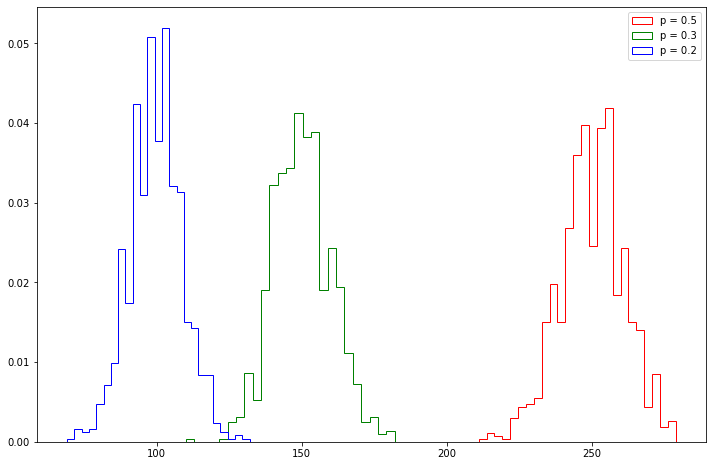
\includegraphics{Figure-15-01}
\end{figure}


\textbf{Exercise 15.6.5 (Computer Experiment)}. Write a function to
generate \(\text{nsim}\) observations from a Multivariate normal with
given mean \(\mu\) and covariance matrix \(\Sigma\).

\textbf{Solution}. Construct our samples based on samples of a
standard multivariate normal \(Z \sim N(0, I)\), by making
\(X = \mu + \Sigma^{1/2} Z\).

\begin{python}
import numpy as np
def multivariate_normal_observations(mu, sigma, nsim=1):
    mu_array = np.array(mu)
    sigma_array = np.array(sigma)
    
    assert len(mu_array.shape) == 1, "mu should be a vector"
    k = mu_array.shape[0]
    
    assert sigma_array.shape == (k, k), "sigma should be a square matrix \ 
                                         with same length as mu"
    
    # Do the eigenvalue decomposition, then get U D^{1/2} as Sigma^{1/2}
    U, D, V = np.linalg.svd(sigma_array)
    sigma_sqrt = U @ np.diag(np.sqrt(D))
    
    # Write our own random normal generator for fun, rather than use np.random.normal
    # Strategy: Use Box-Muller to transform two random uniform variables in (0, 1) 
    # into two standard normals
    def random_normals(size):
        def box_muller(u1, u2):
            R = np.sqrt(-2 * np.log(u1))
            theta = 2 * np.pi * u2
            z0 = R * np.cos(theta)
            z1 = R * np.sin(theta)
            return z0, z1
        def normal_generator(uniform_generator):
            while True:
                z0, z1 = box_muller(next(uniform_generator), next(uniform_generator))
                yield z0
                yield z1
        def random_generator(batch_size):
            while True:
                for v in np.random.uniform(size=batch_size):
                    yield v
        result = np.empty(size)
        gen = normal_generator(random_generator(batch_size=min(size, 1024)))
        for i in range(size):
            result[i] = next(gen)
        return result
    def get_observation():
        z = random_normals(k)
        return mu_array + sigma_sqrt @ z
    
    return np.array([get_observation() for _ in range(nsim)])
\end{python}

\begin{python}
# Sample usage
import matplotlib.pyplot as plt
mu = [1, 3]
sigma = [[2, 1], [1, 2]]
obs = multivariate_normal_observations(mu, sigma, nsim=5000)
plt.figure(figsize=(12, 8))
plt.hexbin(obs[:, 0], obs[:, 1], cmap=plt.cm.Reds)
plt.show()
\end{python}

\begin{figure}[H]
\centering
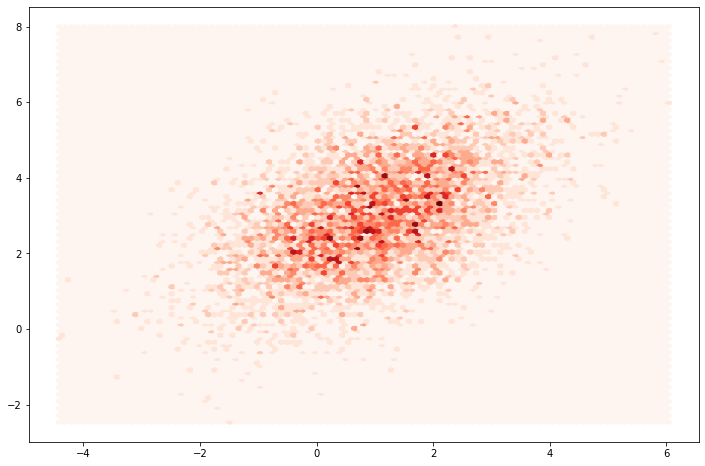
\includegraphics{Figure-15-02}
\end{figure}


\textbf{Exercise 15.6.6 (Computer Experiment)}. Generate 1000 random
vectors from a \(N(\mu, \Sigma)\) distribution where
\[
\mu = \begin{pmatrix} 3 \\ 8\end{pmatrix}
, \quad
\Sigma = \begin{pmatrix}
2 & 6 \\
6 & 2
\end{pmatrix}
\]
Plot the simulation as a scatterplot. Find the distribution of
\(X_{2} | X_{1} = x_{1}\) using Theorem 15.5. In particular, what is the
formula for \(\EXP(X_{2} | X_{1} = x_{1})\)? Plot
\(\EXP(X_{2} | X_{1} = x_{1})\) on your scatterplot. Find the
correlation \(\rho\) between \(X_{1}\) and \(X_{2}\). Compare this with the
sample correlations from your simulation. Find a 95\% confidence
interval for \(\rho\). Estimate the covariance matrix \(\Sigma\).

\textbf{Solution}.
The provided \(\Sigma\) matrix has negative eigenvalues. We will instead
use the following matrix:
\[
\Sigma = \begin{pmatrix} 6 & 2 \\ 2 & 6\end{pmatrix}
\]

\begin{python}
# Generate 1000 vectors
mu = [3, 8]
sigma = [[2, 6], [6, 2]]
obs = multivariate_normal_observations(mu, sigma, nsim=1000)
# Using numpy to generate observations:
#obs = np.random.multivariate_normal(mu, sigma, size=1000)
# Using scipy to generate observations:
#obs = scipy.stats.multivariate_normal.rvs(mean=mu, cov=sigma, size=1000)
x, y = obs[:, 0], obs[:, 1]
# Plot scatterplot
plt.figure(figsize=(12, 8))
plt.scatter(x, y)
plt.show()
\end{python}

\begin{figure}[H]
\centering
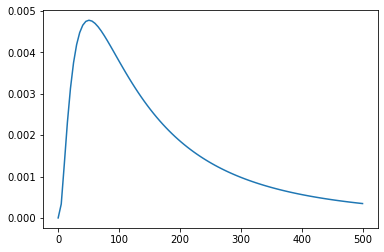
\includegraphics{Figure-12-04}
\end{figure}

From Theorem 15.5,
\[
X_{2} | X_{1} = x_{1} \sim N(\mu(x_{1}), \Sigma(x_{1}))
\]
where
\begin{align*}
\mu(x_{1}) &= \mu_{2} + \Sigma_{21} \Sigma_{11}^{-1} (x_{1} - \mu_{1}) \\
\Sigma(x_{1}) &= \Sigma_{22} - \Sigma_{21}\Sigma_{11}^{-1}\Sigma_{12}
\end{align*}
Replacing the given values,
\begin{align*}
\mu(x_{1}) &= 8 + 2 \cdot 6^{-1} (x_{1} - 3) = \frac{1}{3} x_{1} + \frac{22}{3}\\
\Sigma(x_{1}) &= 6 - 2 \cdot 6^{-1} \cdot 2 = \frac{16}{3}
\end{align*}

\begin{python}
# Plot scatterplot + line
f = lambda x: x/3 + 22/3
plt.figure(figsize=(12, 8))
plt.scatter(x, y)
plt.plot([-6, 10], [f(-6), f(10)], color='red')
plt.show()
\end{python}

\begin{figure}[H]
\centering
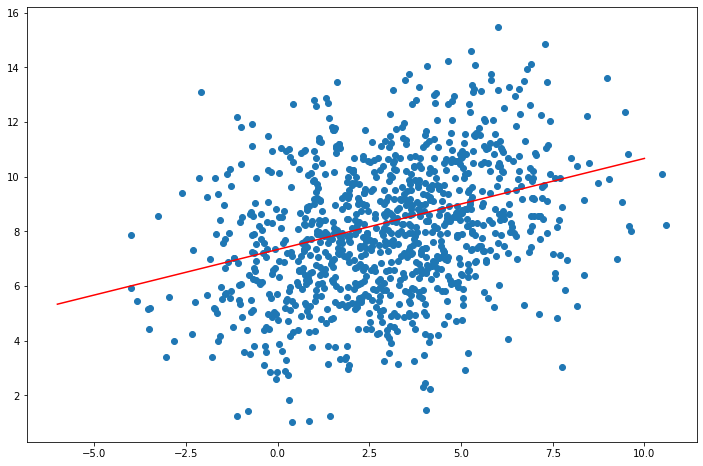
\includegraphics{Figure-15-04}
\end{figure}

The correlation \(\rho\) between \(X_{1}\) and \(X_{2}\) is:
\[
\rho = \frac{\COV(X_{1}, X_{2})}{\sigma_{X_{1}} \sigma_{X_{2}}} = \frac{1}{3}
\]
The estimated correlation \(\rho\) between \(X_{1}\) and \(X_{2}\) is:
\[
\hat{\rho} = \frac{\sum_{i} (X_{1i} - \bar{X}_{1})(X_{2i} - \bar{X}_{2})}{s_{X_{1}} s_{X_{2}}}
\]

\begin{python}
rho_hat = np.corrcoef(x, y)[0, 1]
print("Estimated correlation: %.3f" % rho_hat)
\end{python}
\begin{console}
Estimated correlation: 0.327
\end{console}
We will use the provided process to estimate a confidence interval for
the correlation:
\textbf{Approximate Confidence Interval for the Correlation}
\begin{enumerate}[tightlist,label={\arabic*.}]
\item
  Compute
\end{enumerate}
\[
\hat{\theta} = f(\hat{\rho}) = \frac{1}{2} \left( \log(1 + \hat{\rho}) - \log(1 - \hat{\rho})\right)
\]
\begin{enumerate}[tightlist,label={\arabic*.},resume]
\item
  Compute the approximate standard error of \(\hat{\theta}\) which can
  be shown to be
\end{enumerate}
\[
\widehat{\SE}(\hat{\theta}) = \frac{1}{\sqrt{n - 3}}
\]
\begin{enumerate}[tightlist,label={\arabic*.},resume]
\item
  An approximate \(1 - \alpha\) confidence interval for
  \(\theta = f(\rho)\) is
\end{enumerate}
\[
(a, b) \equiv \left(\hat{\theta} - \frac{z_{\alpha/2}}{\sqrt{n - 3}}, \; \hat{\theta} + \frac{z_{\alpha/2}}{\sqrt{n - 3}} \right)
\]
\begin{enumerate}[tightlist,label={\arabic*.},resume]
\item
  Apply the inverse transformation \(f^{-1}(z)\) to get a confidence
  interval for \(\rho\):
\end{enumerate}
\[
\left( \frac{e^{2a} - 1}{e^{2a} + 1}, \frac{e^{2b} - 1}{e^{2b} + 1} \right)
\]

\begin{python}
from scipy.stats import norm
theta_hat = (np.log(1 + rho_hat) - np.log(1 - rho_hat)) / 2
se_theta_hat = 1 / np.sqrt(1000 - 3)
z = norm.ppf(0.975)
a, b = theta_hat - z * se_theta_hat, theta_hat + z * se_theta_hat
f_inv = lambda x: (np.exp(2*x) - 1) / (np.exp(2*x) + 1)
confidence_interval = (f_inv(a), f_inv(b))
print('95%% confidence interval: %.3f, %.3f' % confidence_interval)
\end{python}
\begin{console}
95\% confidence interval: 0.270, 0.381
\end{console}
The sample covariance matrix is:
\[
\hat{\Sigma} = \frac{1}{n} S = \frac{1}{n} \sum_{i=1}^{n} (X_{i} - \bar{X})(X_{i} - \bar{X})^T
\]

\begin{python}
import numpy as np
mu_hat = np.array([x.mean(), y.mean()])
xx = np.concatenate((x.reshape(-1, 1), y.reshape(-1, 1)), axis=1)
sigma_hat = (xx - mu_hat).T @ (xx - mu_hat) / 1000
sigma_hat
\end{python}
\begin{console}
array([[6.17974344, 1.99813879],
       [1.99813879, 6.05196861]])
\end{console}

\textbf{Exercise 15.6.7 (Computer Experiment)}. Generate 100 random
vectors from a multivariate Normal with mean \((0, 2)^T\) and variance
\[
\begin{pmatrix}
1 & 3 \\
3 & 1
\end{pmatrix}
\]
Find a 95\% confidence interval for the correlation \(\rho\). What is
the true value of \(\rho\)?

\textbf{Solution}.
The provided matrix, yet again, has negative eigenvalues. Instead
use:
\[
\Sigma = \begin{pmatrix}
3 & 1 \\
1 & 3
\end{pmatrix}
\]

\begin{python}
# Generate 100 vectors
n = 100
mu = [0, 2]
sigma = [[3, 1], [1, 3]]
obs = multivariate_normal_observations(mu, sigma, nsim=n)
x, y = obs[:, 0], obs[:, 1]
\end{python}

\begin{python}
# Find 95% confidence interval
from scipy.stats import norm
rho_hat = np.corrcoef(x, y)[0, 1]
theta_hat = (np.log(1 + rho_hat) - np.log(1 - rho_hat)) / 2
se_theta_hat = 1 / np.sqrt(n - 3)
z = norm.ppf(0.975)
a, b = theta_hat - z * se_theta_hat, theta_hat + z * se_theta_hat
f_inv = lambda x: (np.exp(2*x) - 1) / (np.exp(2*x) + 1)
confidence_interval = (f_inv(a), f_inv(b))
print('95%% confidence interval: %.3f, %.3f' % confidence_interval)
\end{python}
\begin{console}
95\% confidence interval: 0.054, 0.424
\end{console}
True value of \(\rho\):
\[
\rho = \frac{\COV(X_{1}, X_{2})}{\sigma_{X_{1}} \sigma_{X_{2}}} = \frac{1}{3}
\]
